\documentclass[11pt, a4paper]{book}
\usepackage[svgnames,table]{xcolor} % For color names
\usepackage{fontspec} % font selecting commands
\usepackage{tcolorbox} % For colored boxes
\usepackage{graphicx} % For pictures
\usepackage[export]{adjustbox}
\usepackage{polyglossia} % Babel alternative in XeLaTex
\usepackage{fancyhdr} % For page headers
\usepackage[top=2.5cm, bottom=2.5cm, left=2cm, right=3cm]{geometry} % To control page margins
\usepackage{listings} % For source code
\usepackage[colorlinks=true,
            urlcolor=blue,
            unicode=true,
            pdftitle={تعلّم البرمجة بلغة الـC},
            pdfauthor={عدن بلواضح,حمزة عباد,أحمد زبوشي}
            pdfdisplaydoctitle=true]{hyperref} % For hyperlinks and PDF metadata
\usepackage{float}
\usepackage{tabu,booktabs}
\usepackage{bidi}
% Language settings
\setmainlanguage[locale=algeria]{arabic}
\setotherlanguage{english}
\addto\captionsarabic{ % Without this, changes won't take effect, because of Polyglossia
  \renewcommand{\partname}{الجزء}
  \renewcommand{\chaptername}{الفصل}
}
% Font settings
\defaultfontfeatures{Ligatures=TeX}
\newfontfamily\arabicfont[Script=Arabic, Scale=1.2]{Amiri} % An arabic font
\newfontfamily\englishfont[Script=Latin]{Arial} % Font used for latin text in the document
\newfontfamily\arabicfonttt{Courier New} % Monospace font, for displaying codes
% Boxes definitions
\tcbset{boxrule=0mm, arc=2pt}
\newtcolorbox{question}{colback=blue!70!green!10, colframe=blue!80!green!5, fontupper=\itshape} % Used for question boxes
\newtcolorbox{critical}{colback=red!20, colframe=red!50} % Used for critical warning boxes
\newtcolorbox{warning}{colback=yellow!20, colframe=yellow!50} % Used for warning boxes
\newtcolorbox{information}{colback=blue!5!green!20, colframe=blue!10!green} % Used for information boxes
\newcommand\InlineCode[1]{\fcolorbox{LightGray}{Snow}{\ttfamily \LR{#1}}}
% Titles settings (Make them orange)
\makeatletter
\let\oldchapter\chapter
\newcommand{\@chapterstar}[1]{\cleardoublepage\phantomsection\addcontentsline{toc}{chapter}{#1}{\color{green!30!blue!80}\oldchapter*{#1}}}
\newcommand{\@chapternostar}[1]{{\color{green!30!blue!80}\oldchapter{#1}}}
\renewcommand{\chapter}{\@ifstar{\@chapterstar}{\@chapternostar}}
\let\oldpart\part
\newcommand{\@partstar}[1]{\cleardoublepage\phantomsection\addcontentsline{toc}{part}{#1}{\color{orange}\oldpart*{#1}}}
\newcommand{\@partnostar}[1]{{\color{orange}\oldpart{#1}}}
\renewcommand{\part}{\@ifstar{\@partstar}{\@partnostar}}
\let\oldsection\section
\newcommand{\@sectionstar}[1]{\phantomsection\addcontentsline{toc}{section}{#1}{\color{orange}\oldsection*{#1}}}
\newcommand{\@sectionnostar}[1]{{\color{orange}\oldsection{#1}}}
\renewcommand\section{\@ifstar{\@sectionstar}{\@sectionnostar}}
\makeatother
% Pictures settings
\graphicspath{{Pictures/}} % Folder of pictures
\newcommand\Picture[2][]{ % This command automatically centers the picture and fits its size to the page. It supports captions too.
  \begin{center}
    \includegraphics[max size={0.8\textwidth}{0.5\textheight}]{#2}\\
    #1
  \end{center}
}
% Paragraphs settings
\setlength{\parskip}{5mm plus2mm minus2mm} % Spacing between paragraphs (+/-)
% Page header and footer settings
\setlength{\headheight}{15pt}
\pagestyle{fancy}
\renewcommand{\chaptermark}[1]{ \markboth{{\thechapter\ #1}}{} }
\renewcommand{\sectionmark}[1]{ \markright{\thesection\ #1} }
\fancyhead{}
\fancyhead[OR,EL]{\rightmark}
\fancyhead[ER,OL]{\leftmark}
\setlength{\footskip}{1.5cm}
% Fixing the issues of the numbering
\renewcommand{\thepart}{\Alph{part}}
\renewcommand{\thechapter}{\Alph{part}.\arabic{chapter}}
\renewcommand{\thesection}{\Alph{part}.\arabic{section}.\arabic{chapter}}
\renewcommand{\thesubsection}{\Alph{part}.\arabic{subsection}.\arabic{section}.\arabic{chapter}}
% C source code
\lstset{language=C, showstringspaces=false, frame=single, numbers=left,
        breaklines=true, keywordstyle=\bfseries\color{Cyan}, commentstyle=\itshape\color{Gray},
        numberstyle=\color{Gray}, stringstyle=\color{Crimson}, basicstyle=\ttfamily,
        morecomment=[l][\color{DarkOrange}]{\#}, showlines, deletekeywords={return,if,else,switch,for,while,do},
        morekeywords=[2]{return,if,else,switch,for,while,do}, keywordstyle=[2]\bfseries\color{Magenta},
        morekeywords=[3]{printf,scanf}, keywordstyle=[3]\color{Cyan}}
\lstnewenvironment{Csource}{\setLTR}{\unsetLTR}
% Table settings
\setlength{\tabulinesep}{2pt}
\setlength{\arrayrulewidth}{2pt}
\taburulecolor{White}
\newenvironment{Table}[1]{ % Accepts 1 parameter which is the number of columns
\taburowcolors[2] 2{LightGray!40 .. LightGray!80}
\begin{center}
  \begin{tabu}{*{#1}{|r}|}
    \toprule
    \rowfont{\bfseries\color{White}}
    \rowcolor{OrangeRed}
    \everyrow{\hline}
}{
  \end{tabu}
\end{center}
}
\newenvironment{Table*}[1]{
\taburowcolors[1] 2{LightGray!40 .. LightGray!80}
\begin{center}
  \begin{tabu}{*{#1}{|r}|}
    \toprule
    \everyrow{\hline}
}{
  \end{tabu}
\end{center}
}

\title{تعلّم البرمجة بلغة الـC}
\begin{document}
  \chapter*{تقديم}
إن التحرّر الفكري في بداية القرن العشرين أدّى إلى توسّع في البحوث العلمية التي شملت كل الميادين لاسيّما التكنولوجية منها كعلوم الحاسوب. هذه الأخيرة أعقبتها ثورة في لغات البرمجة التي تعتبر ركيزة أساسية تقوم عليها البرامج. من بين هذه اللغات نجد لغة الـ\textenglish{C}،
إذ تعتبر من أقوى لغات البرمجة و أكثرها شيوعاً، فهي مستلهمة من طرف لغتي
 \textenglish{B}
 و
 \textenglish{BCPL}
حيث تمّ تطويرها في عام 1972 من طرف
\textenglish{Ken Thompson}
و
 \textenglish{Dennis Ritchie}،
و في ظرف سنة واحدة توسّعت لتكون عِـماد نظام التشغيل
\textenglish{UNIX}
بنسبة
90\%
ثم تم توزيعها في العام المـُوالي رسمياً عبر الجامعات لتصبح بذلك لغة برمجة عالمية. و اشتهرت لغة الـ\textenglish{C}
 كونـُها لغة عالية المستوى، لها مُترجم سريع و فعّال. كما أنها لغة برمجية نقّالة، هذا يعني أن أي برنامج يحترم المعيار
\textenglish{AINSI}
يمكن أن يتمّ تشغيله على أيّة منصّة تحتوي على مترجم
\textenglish{C}
 دون أيّة تخصيصات.

يعتبر هذا الكتاب بوابة سهلة لكلّ مبتدئ لتعلّم لغة الـ\textenglish{C}
خطوة بخطوة بدءً من الأساسيات وصولاً إلى تطوير ألعاب ثنائية الأبعاد و التحكّم في هياكل البيانات الأكثر تعقيداً. الكتاب مرفق بجملة من التمارين و الأعمال التطبيقية المحلولة التي تساعد على هضم المفاهيم المكتسبة و تطبيقها على أيّ مشكل برمجي مهما كان نوعه. و لأن الكثير من لغات البرمجة تعتمد أساساً على الـ\textenglish{C}
كالـ\textenglish{Java}
و الـ\textenglish{C++}\chapter*{تقديم}
إن التحرّر الفكري في بداية القرن العشرين أدّى إلى توسّع في البحوث العلمية التي شملت كل الميادين لا سيّما التكنولوجية منها كعلوم الحاسوب. هذه الأخيرة أعقبتها ثورة في لغات البرمجة التي تعتبر ركيزة أساسية تقوم عليها البرامج. من بين هذه اللغات نجد لغة \textenglish{C}،
إذ تعتبر من أقوى لغات البرمجة وأكثرها شيوعًا، فهي مستلهمة من طرف لغتي
 \textenglish{B}
 و
 \textenglish{BCPL}
حيث تمّ تطويرها في عام 1972 من طرف
\textenglish{Ken Thompson}
و
 \textenglish{Dennis Ritchie}،
و في ظرف سنة واحدة توسّعت لتكون عِـماد نظام التشغيل
\textenglish{UNIX}
بنسبة
90\%
ثم تم توزيعها في العام المـُوالي رسميًا عبر الجامعات لتصبح بذلك لغة برمجة عالمية. واشتهرت لغة \textenglish{C}
 كونـُها لغة عالية المستوى، لها مُترجم سريع و فعّال. كما أنها لغة برمجية نقّالة، هذا يعني أن أي برنامج يحترم المعيار
\textenglish{AINSI}
يمكن أن يتمّ تشغيله على أيّة منصّة تحتوي على مترجم
\textenglish{C}
 دون أيّة تخصيصات.

يعتبر هذا الكتاب بوابة سهلة لكلّ مبتدئ لتعلّم لغة \textenglish{C}
خطوة بخطوة بدءً من الأساسيات وصولًا إلى تطوير ألعاب ثنائية الأبعاد والتحكّم في هياكل البيانات الأكثر تعقيدًا. الكتاب مرفق بجملة من التمارين والأعمال التطبيقية المحلولة التي تساعد على هضم المفاهيم المكتسبة وتطبيقها على أيّ مشكل برمجي مهما كان نوعه. ولأن الكثير من لغات البرمجة تعتمد أساسًا على \textenglish{C}
مثل \textenglish{Java}
و \textenglish{C++}
و \textenglish{C\#}
(لغات برمجية غرضية التوجّه) وحتى
\textenglish{PHP}
(لغة لبرمجة المواقع) فإن تعلّم لغة \textenglish{C}
 سيساعد على تعلّم أيّة لغة برمجية كانت. تبقى الإرادة وحبّ العمل والشغف المفاتيح الرئيسية للنجاح والوصول إلى الاحترافية.

\vfill

\hfill\parbox{0.3\textwidth}{\centering
عدن بلواضح

\vspace{1em}
الجزائر\\[0.5em]
في
24 ذو القعدة 1438\\[0.3em]
الموافق لـ17 أوت 2017
%\Hijritoday\\[0.3em]
%الموافق لـ\today

}


و الـ\textenglish{C\#}
(لغات برمجية غرضية التوجّه) و حتى
\textenglish{PHP}
(لغة لبرمجة المواقع) فإن تعلّم لغة الـ\textenglish{C}
 سيساعد على تعلّم أيّة لغة برمجية كانت. تبقى الإرادة و حبّ العمل و الشغف المفاتيح الرئيسية للنجاح و الوصول إلى الاحترافية.

\vfill

\hfill\parbox{0.3\textwidth}{\centering
عدن بلواضح

\vspace{1em}
الجزائر\\[0.5em]
في
24 ذو القعدة 1438\\[0.3em]
الموافق لـ17 أوت 2017
%\Hijritoday\\[0.3em]
%الموافق لـ\today

}


  \part{أساسيّات البرمجة بلغة الـC}
  \chapter{قلت برمجة ؟}
\section{ما هي البرمجة؟}
\begin{question}
  ما الذي تعنيه كلمة "بَرْمَجَ"؟
\end{question}

لن أتعبك وأعطيك أصل كلمة "بَرْمَجَ"، لكنني سأختصر كل شيء في جملة: البرمجة تعني إنشاء برامج حاسوب. وهذه البرامج التي تنشئها تأمر الجهاز بالقيام بتعليمات وأفعال معيّنة.
حاسوبك الخاص يحتوي على كثير من هذه البرامج وبمختلف أنواعها:

\begin{itemize}
  \item الآلة الحاسبة تعتبر برنامجاً.
  \item معالج النصوص يعتبر برنامجاً أيضاً.
  \item وكذلك برنامج المحادثة.
  \item ألعاب الفيديو هي برامج كذلك.
\end{itemize}

\Picture[\caption{نسخة عن لعبة \textenglish{MetalSlug} الشهيرة تم إنشاؤها من طرف العضو \href{http://www.siteduzero.com/membres-294-176405.html}{\textenglish{joe87}}}]{Chapter_I-1_MetalSlug}
باختصار البرامج موجودة في كل جهاز، وهي التي تعطي الحاسوب قدرته على إنجاز مختلف المهام التي تُخوَّل إليه. يمكنك أن تنشئ برنامج تشفير أو لعبة ثنائية / ثلاثية الأبعاد باستخدام لغة برمجة مثل \textenglish{C}.

ملاحظة: لم أقل أن إنشاء لعبة يتم برمشة عين، لقد قلت فقط بأنه شيء ممكن، لكن كن متأكداً، سوف يتطلب ذلك جهدا كبيراً!

وبما أننا في بداية الطريق، فإّننا لن نقوم بإنشاء لعبة ثلاثية الأبعاد! لكنّنا سنبدأ بكيفية عرض نص على الشاشة، طبعا ستقول ما علاقة هذا بإنشاء الألعاب؟ لكن ثِق بي، هذا الأمر ليس بسيطا كما يبدو!

بالطبع هذا ليس شيئا مُبهراَ، ولكن يجب علينا أن نبدأ من هنا؛ وشيئا فشيئا يمكنك أن تنشئ برامج معقّدة أكثر. فالهدف من هذا الدرس هو أن أعرفك على كل ما يتعلق بهذه اللغة.

\section{البرمجة، بأي لغة يا ترى؟}
حاسوبك هو آلة غريبة جداً، هذا أقل ما يمكن أن نقوله عنه. يمكننا أن نخاطبه فقط بالصفر والواحد، فمثلا إذا طلبنا منه حساب 3+5 فيمكن لهذا أن يعطينا نتيجة كالتالي (هذه ليست ترجمة دقيقة ولكنها تشبه ما يحدث بالفعل):\\
\InlineCode{0010110110010011010011110}

ما تَرَاه هنا يسمى اللغة الثنائية
(\textenglish{Binary language})
أو لغة الآلة
(\textenglish{Machine language})،
وحاسوبك لا يفهم سوى هذه اللغة، وكما تلاحظ، هذه اللغة غير مفهومة على الإطلاق!

مشكلتنا الآن:
\begin{question}
  كيف يمكننا التعامل مع حاسوب لا يفهم سوى اللغة الثنائية؟
\end{question}

حاسوبك لا يتحدث الإنجليزية، ولا العربية، ولا أي لغة غير هذه اللغة، ولكنها صعبة جدا لدرجة أن حتى أكبر خبراء الحاسوب لا يستخدمونها.
لهذا قام بعض مهندسي الحواسيب باختراع لغات يمكن أن تُتَرجَمَ إلى اللغة الثنائية، لكن الشيء الأصعب هو إنشاء البرامج الّتي تقوم بهذه الترجمة. ولحسن الحظ فقد قاموا بهذا العمل نيابة عنا. هذه البرامج تقوم بترجمة الأوامر الّتي تكتبها (مثلا: "أُحسب 3+5") إلى شيء يشبه هذا:
\InlineCode{0010110110010011010011110}.

هذا المخطط يلخص ما كنت أشرح:

\Picture{Chapter_I-1_Translation}

\section{قليل من المفردات}
حتّى الآن كنت أتحدّث إليك بكلمات بسيطة، لكن يجب أن تعلم أنه في المعلوماتية توجد مصطلحات علمية لكل ما ذكرت. طوال هذا الدرس، سوف تتعلم استخدام المفردات المناسبة. هذا سيفيدك كثيرا خصوصا عندما تتحدث مع مبرمجين آخرين، حيث أنك سوف تتفاهم معهم بكل سهولة.

نعود إلى الحديث عن المخطط السابق في المستطيل الأول قلت أن "برنامجك مكتوب بلغة مُبَسَّطة"، في الواقع هذا النوع من اللغات يُعرف باسم لغات البرمجة عالية المستوى (\textenglish{High-level programming languages}). هناك مستويات عديدة من لغات البرمجة، وكلما كان مستوى اللغة أعلى كانت أقرب إلى اللغة الحقيقية وكان استخدامها أسهل. إذن، اللغات عالية المستوى سهلة الاستخدام لكنها تتضمن بعض السلبيّات سوف نتعرّف عليها لاحقا.

توجد العديد من لغات البرمجة، وهي متفاوتة المستوى، منها:
\begin{itemize}
  \item \textenglish{C}
  \item \textenglish{C++}
  \item \textenglish{Java}
  \item \textenglish{Visual Basic}
  \item \textenglish{Delphi}
  \item و العديد غيرها
\end{itemize}

كما تلاحظ، لم أرتبها حسب مستوياتها، لذلك لا تعتقد أن اللغة الأولى في القائمة هي الأسهل أو العكس. عموما، لائحة اللغات الموجودة طويلة جدا لدرجة أنه لا يمكنني كتابتها كلها هنا.

مصطلح آخر يجب تذكّره هو
\underline{الشفرة المصدرية}
(\textenglish{Source code})،
 وهي ببساطة الشفرة الخاصة ببرنامجك الذي تكتبه بلغة عالية المستوى والذي يتم ترجمته فيما بعد إلى اللغة الثنائية.

 ثم يأتي دور البرنامج الذي يحوّل هذه اللغة عالية المستوى إلى اللغة الثنائية، هذا النوع من البرامج يعرف باسم
 \underline{المترجم}
  أو
  \underline{المصنّف}،
 والعملية الّتي يقوم بها تسمى
 \underline{الترجمة}
 أو
 \underline{التصنيف}.

\begin{information}
  يوجد لكل لغة عالية المستوى مترجم خاص، وهذا شيء منطقي، فاللغات مختلفة فيما بينها، فلا يمكننا ترجمة لغة
\textenglish{C}
بنفس الطريقة الّتي نترجم بها
\textenglish{Delphi}
مثلا.
  بعض اللغات مثل
\textenglish{C}
تملك العديد من المترجمات، فمنها من هو مكتوب من طرف
\textenglish{Microsoft}
، و منها من
\textenglish{GNU}
، إلخ… سوف نتعرّف على كل هذا في الدرس القادم.
  لحسن الحظ، هذه المترجمات متطابقة تقريبا (رغم وجود اختلافات طفيفة بينها سوف نتعرف عليها لاحقا).
\end{information}

أخيرا، البرنامج الثنائي المنشئ بواسطة المترجم يسمى الملف
\underline{القابل للتنفيذ}
أو
\underline{التنفيذي}
(\textenglish{Executable}).
 لهذا السبب تملك البرامج
 (على الأقل برامج
 \textenglish{Windows})
 الامتداد
\textenglish{.exe}
 والذي هو اختصار كلمة
 \textenglish{EXEcutable}.

 نعود إلى مخططنا السابق، وهذه المرة سنستخدم المصطلحات الصحيحة:

 \Picture{Chapter_I-1_Compilation}

 \section{لماذا نختار تعلّم \textenglish{C}؟}
 كما قلت سابقا، يوجد كثير من اللغات عالية المستوى، فلماذا ينبغي علينا أن نبدأ بإحداها على وجه الخصوص؟ سؤال عظيم!

على أية حال يجب علينا أن نختار بأي لغة سنبدأ البرمجة عاجلا أم آجلا، وبالتالي لديك الخيار في البدء بـ:
\begin{itemize}
  \item \textbf{لغة ذات مستوى عالي جدّا}:
 وتكون سهلة جدّا أوعامة، نذكر من بينها
 \textenglish{Python}، \textenglish{Ruby}، \textenglish{Visual Basic}،
 وغيرها. هذه اللغات تسمح بكتابة برامج بشكل أسرع. عامّة تحتاج لأن تُرفق معها ملفات مُسَاعِدة لكي تعمل (كَمُفَسِّرٍ مثلا).
  \item \textbf{لغة ذات مستوى منخفض قليلا}:
هي أكثر صعوبة نوعا ما، ولكن مع لغة مثل
\textenglish{C}
 سوف تتعلم كثيرا عن البرمجة وحول طريقة عمل حاسوبك. ستكون بعد ذلك قادراً على تعلّم لغة برمجة أخرى إن أردت وبكل يُسْرٍ.
\end{itemize}

من ناحية أخرى،
\textenglish{C}
لغة برمجة واسعة الإنتشار، أُستخدمت في برمجة العديد من البرامج التي تعرفها. حتى أنها كثيرا ما تدرّس في الدراسات العليا في مجال المعلوماتية.
هذه هي الأسباب الّتي جعلتني أتحمّس لتعليمك لغة
\textenglish{C}
بالتحديد. لم أقل أنّه يجب عليك أن تبدأ بها، لكنّي قلت إنه خيار جيّد لكي أقدّم لك معرفة صلبة في هذا الدرس.

\begin{information}
  بعض لغات البرمجة موجّهة أكثر للشبكة العنكبوتية
 (\textenglish{Web})
 مثل
 \textenglish{PHP}
 أكثر منها من إنشاء البرامج المعلوماتية.
\end{information}

سوف أفترض في هذا الكتاب أنّ هذه هي لغة برمجتك الأولى وأنّه لم يسبق لكم أن برمجت من قبل. فإن كنت قد برمجت قليلا من قبل فلا مضرّة في أن تعيد من الصفر.

\begin{question}
  ما هو الفرق بين
  \textenglish{C}
  و
  \textenglish{C++}
  ؟
\end{question}

هاتان اللغتان قريبتان جدّا من بعضهما، وكلاهما مستخدمتان بكثرة. ولكي تعرف كيف نشأتا يجب عليك أن تدرس التاريخ قليلا:
\begin{itemize}
  \item في البداية، عندما كانت الحواسيب تَزِنُ أطنانا وتشغل مكانا قَدْرُهُ حجم منزلك، تمّ إختراع لغة برمجة تسمّى
\textenglish{Algol}.
  \item بعدها تطوّرت الأمور أكثر واختُرعَت لغة برمجة جديدة عُرِفَتْ باسْمِ
\textenglish{CPL}
 والّتي تطوّرت فيما بعد إلى لغة
\textenglish{BCPL}
 ثم أخذت إسم اللغة
\textenglish{B}.
  \item مع مضيّ الزمن توصّل الخبراء إلى ابتكار اللغة
\textenglish{C}
 وقد تمّ إدخال بعض التعديلات عليها إلّا أنها لا تزال من أحد اللغات الأكثر استخداما اليوم.
  \item وبعد زمن، أراد الخبراء أن يضيفوا بعض الأشياء إلى
\textenglish{C}
، يمكن اعتبارها نوعا من التحسينات. والنتيجة كانت بما يعرف بلغة
\textenglish{C++}
، وهي لغة
\textenglish{C}
 مع إضافات تمكّننا من البرمجة بطريقة مختلفة.
\end{itemize}

\begin{information}
  الـ
\textenglish{C++}
ليست أحسن من الـ
\textenglish{C}
، هي فقط تمكننا من البرمجة بطريقة مختلفة وتساعد المبرمج على تنظيم شفرة برنامجه. رغم ذلك هي تشبه الـ
\textenglish{C}
كثيرا. وإن كنت تنوي تعلّم الـ
\textenglish{C++}
فيما بعد فَسَوْفَ تجد ذلك سهلا.
\end{information}

ولو اعتُبرت
\textenglish{C++}
 تطويرا لـ
\textenglish{C}
 فإن هذا لا يعني أنه يجب استخدام
\textenglish{C++}
 فقط لإنشاء البرامج. لغة
\textenglish{C}
 ليست لغة عجوزا منسيّة، بالعكس هي مستخدمة بكثرة اليوم. بل إنها أساس أنظمة التشغيل الكبيرة مثل
\textenglish{Unix }
(ومنه
\textenglish{GNU/Linux}
 و
\textenglish{Mac OS}) و
\textenglish{Windows}.

\section{هل البرمجة صعبة؟}
هذا سؤال يعذّب روح كل من يريد تعلّم البرمجة! هل يجب أن تكون أستاذ رياضيات كبير درس 10 سنوات من التعليم العالي حتّى تبدأ البرمجة؟

الجواب هو لا بالطبع. كل ما تحتاج إليه هو معرفة العمليات الأربع الأساسية:
\begin{itemize}
  \item الجمع
  \item الطرح
  \item الضرب
  \item القسمة
\end{itemize}
هذا ليس مخيفا! سوف أشرح لك في درس لاحق كيف يقوم الحاسوب بهذه العمليات الأساسية في برامجك.

باختصار، لا توجد صعوبات غير قابلة للحلّ. في الواقع، هذا يعتمد على طبيعة برنامجك، فإذا كنت تريد إنشاء برنامج تشفير فيجب عليك معرفة بعض الأشياء في الرياضيات، وإن كان برنامجك يقوم بالرسم ثلاثي الأبعاد فيجب أن تكون لديك بعض المعرفة بالهندسة الفضائية.

كل حالة تعامل بطريقة خاصّة. ولكن لتعلّم لغة
\textenglish{C}
 نفسها لا تحتاج إلى أيّة معارف قبليّة.

\begin{question}
  إذن أين هو الفخ؟ وأين تكمن الصعوبة؟
\end{question}

يجب أن تعرف كيف يعمل الحاسوب، لتفهم ما الّذي نقوم به في C. من هذا المنطلق، كن متيقّنا أنّي سأعلّمك كلّ هذا شيئا فشيئا.

اعلم أن للمبرمج صفات أيضا مثل:
\begin{itemize}
  \item الصبر: البرنامج لا يعمل عادة من أوّل محاولة، يجب أن تكون مثابراً.
  \item حسّ المنطق: صحيح أنّك لست بحاجة إلى أن يكون لديك مستوى جيّد في الرياضيّات، لكنّ هذا لا يمنع من التفكير وتحليل المشكلات بالمنطق.
  \item الهدوء: فيجب عليك ألّا تضرب حاسوبك بالمطرقة، فهذا لن يجعل برنامجك يعمل!
\end{itemize}

  \chapter{برنامجك الأوّل}

لقد قمنا بتحضير كلّ شيء إلى حد الآن ويمكننا أن نبدأ قليلا من البرمجة. مع نهاية هذا الفصل ستكون قد نجحت في إنشاء أوّل برنامج لك.

لكي أصدقك القول، سيظهر البرنامج بالأبيض والأسود ولن يقوم بشيء سوى إلقاء التحيّة. يبدو عديم الفائدة، لكنّه برنامجك الأوّل وأؤكّد لك أنّك ستكون فخورا به.

\section{كونسول أو نافذة ؟}

لقد تحدثنا سابقا عن فكرة برامج الكونسول وبرامج النوافذ في الفصل السابق. البيئة التطويرية تطلب منا تحديد أي نوع من البرامج نريد أن ننشئها. ولقد قلنا إننا سننشئ برامج من نوع كونسول.

يوجد نوعان من البرامج، لا أكثر :

\begin{itemize}
  \item ،برامج بنوافذ
  \item برامج تعمل في الكونسول.
\end{itemize}

\subsection{البرامج الّتي تملك نوافذ}

هي البرامج التي نعرفها جميعا. هذا مثال على برنامج من نوع نافذة، مثل الرسام.

\begin{figure}[H]
	\centering
	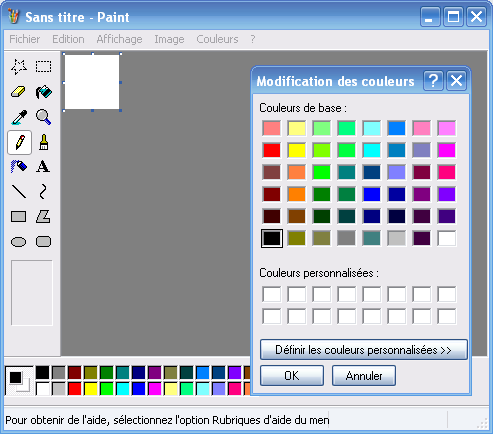
\includegraphics[width=0.6\textwidth]{Chapter_I-3_Paint}
\end{figure}

أعتقد أنّك تحب إنشاء برامج كهذه، لكنّ هذا ليس في مقدورك حاليا. في الواقع، إنشاء برامج بنوافذ هو أمر ممكن بلغة \textenglish{C}، لكنّ بالنسبة لمبتدئ، هذا أمر معقّد جدّا. كبداية، يستحسن إنشاء برامج الكونسول.

\begin{question}
  لكن ماذا يعنى برنامج
\textenglish{Console}
؟
\end{question}

\subsection{البرامج الّتي تعمل في الكونسول}

برامج الكونسول هي أول ما ظهر من برامج. في ذلك الوقت، شاشات الحواسيب لم تكن سوى بالأبيض والأسود، ولم تكن فعّالة لكي تتمكّن من رسم النوافذ كما هو الحال مع حواسيبنا حاليّا.

مرّ الزمن بسرعة وزادت شعبية الويندوز نظراً لبساطته إلى أن نسي كثير من الناس ما هي الكونسول.

لديّ خبر جيّد لك !
\textbf{الكونسول لم تمت بعد} !
 في الواقع،
\textenglish{GNU/Linux}
 قد أعاد الكونسول إلى الحياة. هذه صورة لكونسول على
\textenglish{GNU/Linux}.

\begin{figure}[H]
	\centering
	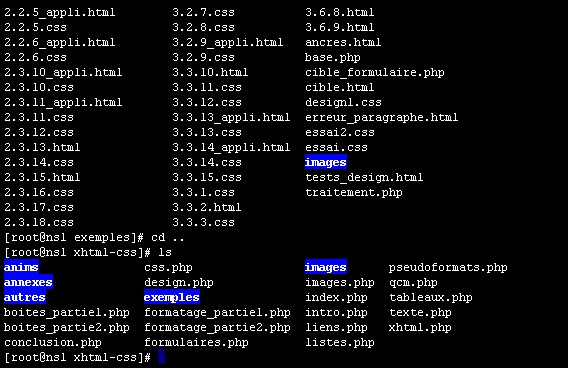
\includegraphics[width=0.6\textwidth]{Chapter_I-3_Console}
\end{figure}

مرعب ! صحيح ؟ لكن على الأقل عرفت ما هي الكونسول، وهذه بعض الملاحظات :

\begin{itemize}
  \item اليوم، يمكننا عرض الألوان في الكونسول. ليس كلّ شيء بالأبيض والأسود كما تتخيّل.
  \item الكونسول هو الأسهل من ناحية البرمجة بالنسبة للمبتدئين.
  \item أداة عالية الإمكانيّات إذا عرفنا كيف نستخدمه.
\end{itemize}

كما قلت لك، إنشاء برامج كونسول أمر سهل جدّا وملائم للمبتدئين (وهذا عكس برامج النوافذ). ليكن في علمك أيضا أنّ الكونسول قد تطوّرت وبإمكانها عرض الألوان، ولا شيء يمنعك من إضافة صورة خلفيّة لها.

\begin{question}
  وفي الويندوز ألا توجد
\textenglish{Console}
 ؟
\end{question}

بلى، لكنّها مخفيّة لو صح القول. يمكنك فتحها بالذهاب إلى "إبدأ"
(\InlineCode{Start})
 ثمّ "ملحقات"
(\InlineCode{Accessories})
 ثمّ "موجه الأوامر"
(\InlineCode{Command prompt})
 أو بالذهاب إلى "إبدأ" ثمّ "تشغيل"
(\InlineCode{Run})
 واكتب فيها
\InlineCode{cmd}
 واضغط على "موافق".

\begin{figure}[H]
	\centering
	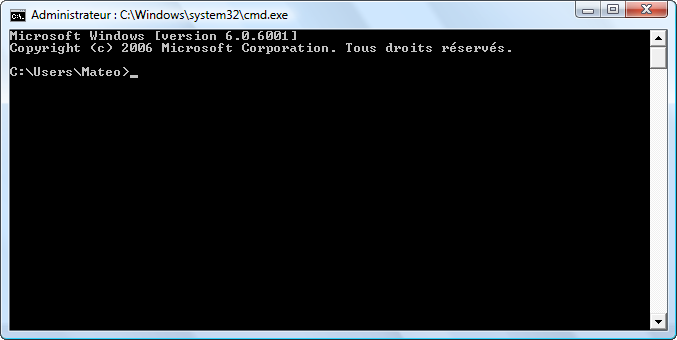
\includegraphics[width=0.6\textwidth]{Chapter_I-3_Console-Windows}
\end{figure}

إذا كنت تستخدم نظام ويندوز، فاعلم بأن أولى برامجك ستكون في نوافذ شبيهة بهذه. أنا لم أختر البداية هكذا لجعلك تشعر بالملل، بل لتعليمك الأساسيّات اللازمة لكي تتمكّن لاحقا من إنشاء النوافذ.

إذن فلتكن متيقّناً، بمجرّد أن تصل إلى المستوى اللازم لإنشاء النوافذ، سوف أعلّمك كيف تفعل ذلك.

\section{الحدّ الأدنى من الشفرة المصدرية}

من أجل أي برنامج، يجب كتابة قدر معيّن من الشفرة المصدرية. هذه الشفرة لا تقوم بشيء خاصّ لكنّها ضروريّة. هذه الشفرة التي سنكتشفها الآن ستكون أساس أغلب برامجك الّتي ستكتبها بلغة \textenglish{C}.

\subsection{أطلب من البيئة التطويرية الخاصة بك تزويدك بالحد الأدنى من الشفرة المصدرية}

لقد لاحظت أن طريقة إنشاء مشروع جديد تختلف من بيئة تطويرية إلى أخرى. إليك تذكيراً بسيطا : في برنامج
\textenglish{Code::Blocks}
 (الذي سنستخدمه في هذا الكتاب)، عليك التوجه نحو
\InlineCode{File}
 ثمّ
\InlineCode{New}
 ثمّ
\InlineCode{Project}
 ثم تختار
\InlineCode{Console Application}
 وبعدها اللغة
\textenglish{C}.
سيولّد لك الحد الأدنى من الشفرة المصدرية
 \textenglish{C}
 التي تحتاجها. ها هي :

\begin{Csource}
#include <stdio.h>
#include <stdlib.h>

int main()
{
    printf("Hello world!\n");
    return 0;
}

\end{Csource}

\begin{information}
لاحظ أنّه يوجد سطر فارغ في نهاية الشفرة. يفترض أن ينتهي كل ملف مكتوب بلغة
\textenglish{C}
هكذا. إن لم تفعل ذلك، فهذه ليست بمشكلة، لكن توقّع أن يعرض لك المترجم تحذيراً
(\textenglish{Warning}).
\end{information}

علماً أنّ السطر :
\begin{Csource}
int main()
\end{Csource}
\dots
بإمكانه أن يُكتب كالتالي :

\begin{Csource}
int main(int argc, char *argv[])
\end{Csource}

كلتا العبارتين تحملان نفس المعنى لكن الثانية، الأكثر تعقيدا، هي الأكثر شيوعا، لذلك فإنّنا سنستخدمها في الفصول القادمة.\\
إستخدامنا للشكل الأوّل أو الثاني لا يغيّر شيئا بالنسبة لنا. لذلك لا داعي لإضاعة الوقت هنا، خصوصاً أنّك لا تملك المستوى اللازم لفهم ما تعنيه.

إذا كنت تستخدم بيئة تطويرية أخرى فقم بنسخ هذه الشفرة المصدرية وألصقها في الملف \InlineCode{main.c} ليكون لديكم نفس الشفرة.

أخيرا، قم بحفظ عملك في المشروع. أعلم أننا لم نقم بشيء حتّى الآن لكن من الجيّد التعوّد على الحفظ في كلّ مرّة.

\subsection{تحليل أسطر الشفرة المصدرية السابقة}
قد تبدو لك الشفرة المصدرية السابقة أنّها كاللغة الصينيّة، أنا أتخيّل ذلك ! في الواقع هي تسمح بإنشاء برنامج كونسول يعرض نصّا على الشاشة. يجب تعلّم كيفيّة قراءة كلّ هذا.

فلنبدأ بأوّل سطرين :
\begin{Csource}
#include <stdio.h>
#include <stdlib.h>
\end{Csource}

هذان السطران يبدآن بعلامة
\InlineCode{\#}.
وهي أسطر خاصّة تُعرف باسم
\textbf{توجيهات المعالج القبلي}
(\textenglish{Preprocessor directives}). اسم معقّد، أليس كذلك ؟ هذه الأسطر تتمّ قراءتها من طرف البرنامج المسمّى بالمعالج القبلي، وهو برنامج يتمّ تشغيله في بداية الترجمة.

ما رأيناه سابقا كان مخطّطا بسيطا لعمليّة الترجمة. لكنّ في الواقع، هناك الكثير من المراحل التي تحدث في هذه العمليّة. سنقوم بتفصيل هذا لاحقا. حاليّا عليك فقط تذكّر وضع هذين السطرين أعلى كلّ ملفّاتك.

\begin{question}
  حسنا لكن ماذا يعنيه هذان السطران ؟ أريد أن أعرف !
\end{question}

كلمة
 \InlineCode{include}
 بالإنجليزيّة تعني "تضمين". هذان السطران يقومان بتضمين ملفّات في المشروع، أي إضافة هذه الملفّات من أجل عمليّة الترجمة. هناك سطران وبالتالي هناك ملفان يتمّ تضمينهما في المشروع وهما بالترتيب :
\InlineCode{stdio.h}
 و
\InlineCode{stdlib.h}.
هذان الملفّان موجودان بالفعل على حاسوبك وهما ملفّان مصدريّان جاهزان، سوف تعرف مستقبلا أنّنا نسميها
\textbf{مكتبات}
(\textenglish{Libraries}).
 هذه الملفّات تحتوي الشفرة المصدرية اللازمة لعرض نصّ على الشاشة.

 بدون هذين الملفّين، كتابة نصّ على الشاشة سيكون أمرا مستحيلاً. فالحاسوب لا يعرف فعل أي شيء مبدئيا.

 باختصار، السطران الأول والثاني يقومان بتضمين المكتبات التي ستساعدنا في إظهار نصّ على الشاشة بكلّ سهولة.

 نمر للتالي، باقي الأسطر :
 
\begin{Csource}
int main()
{
    printf("Hello world!\n");
    return 0;
}
\end{Csource}

ما تراه هنا هو ما نسميه بـ\textbf{التابع}
أو
\textbf{الدالّة}
(\textenglish{Function}).
 البرنامج في لغة
\textenglish{C}
 يتكوّن من مجموعة دوال. حاليّا برنامجنا لا يحوي سوى دالّة واحدة.

الدالّة تمكّننا من تجميع مجموعة من الأوامر. الغرض من تجميع الأوامر هو جعلها تقوم بوظيفة ما. مثلا يمكننا إنشاء دالّة باسم
 \InlineCode{open\_file}
 وجعلها تحتوي التعليمات التي تشرح للحاسوب كيفيّة فتح ملف.

 دون الدخول في تفاصيل إنشاء الدالّة (الوقت مبكّر، سوف نتحدّث عن الدوال في وقت لاحق) لنحلّل رغم ذلك أجزائه الكبيرة. السطر الأوّل يحتوي اسم الدالّة، إنّه الكلمة الثانية.\\
 أجل، اسم دالّتنا هو
\InlineCode{main}
والذي يعني
"الرئيسية"
. وتشغيل البرنامج دائما يبدأ من الدالة
\InlineCode{main}.

للدالّة بداية ونهاية، وهي محدودة بالحاضنتين
\InlineCode{\{}
و
\InlineCode{\}}.
محتوى الدالّة موجود بين هاتين الحاضنتين. إن كنت قد تابعت جيداً فقد عرفت أنّ الدالّة مشكّلة من سطرين :

\begin{Csource}
printf("Hello world!\n");
return 0;
\end{Csource}

هاته الأسطر في الداخل نسميها
\textbf{التعليمات}
(\textenglish{Instructions})
 (هذه إحدى المصطلحات الّتي يجب عليك حفظها). كلّ تعليمة تمثّل أمراً بالنسبة للحاسوب. فكلّ واحدة منها تطلب منه فعل شيء محدّد.

 كما قلت لك، بتجميع ذكيّ للتعليمات في الدالّة يمكننا إنشاء أجزاء برنامج جاهزة للاستخدام. باستخدام التعليمات المناسبة يمكننا إنشاء دالّة
 \InlineCode{open\_file}
 كما شرحت لك قبل قليل، و أيضا دالّة
\InlineCode{move\_character}
 في لعبة فيديو، على سبيل المثال.

 البرنامج في الواقع ما هو إلّا تتابع لتعليمات : إفعل هذا و إفعل ذاك. أنت تعطي أوامر للحاسوب و هو يقوم بتنفيذها.

 \begin{critical}
هامّ جدّا : لا بدّ أن تنتهي كلّ تعليمة بفاصلة منقوطة
"\InlineCode{;}"
. بهذا يمكن التفريق بين ما إذا كانت هذه تعليمة أم لا. إذا نسيت وضع فاصلة منقوطة نهاية تعليمة ما، فلن تتمّ ترجمة برنامجك.
 \end{critical}

 السطر الأول :
 \InlineCode{printf("Hello world!\\n");}
 يطلب إظهار الرسالة
 "\textenglish{Hello world!}"
  على الشاشة. عندما يصل برنامجك إلى هذا السطر، فسوف يقوم بعرض هذه الرسالة ثمّ المرور إلى التعليمة التالية.

  التعليمة التالية هي
\InlineCode{return 0;}
 و هي تخبرنا أنّ الدالّة
\InlineCode{main}
 قد انتهت و تطلب منه إعادة 0.

 \begin{question}
   لماذا يقوم برنامجي بإعادة العدد 0 ؟
 \end{question}

 في الواقع، كلّ برنامج عندما ينتهي يُرجع قيمة معينة. على سبيل المثال، ليقول أنّ كلّ شيء سار على ما يرام. عمليّا، 0 يعني  أنّ كلّ شيء سار على ما يرام، و كلّ قيمة أخرى تدلّ على حدوث خطأ. في أغلب الأحيان هذه القيمة لا تُستخدم ، لكن يجب رغم ذلك استعمالها.\\
 كان يمكن أن يعمل برنامجك بدون
 \InlineCode{return 0}
، لكن يمكننا القول أن وضعها يعتبر أمراً أكثر نظافة و أكثر جدّية.

إلى هنا نكون قد فصّلنا قليلا في عمل هذه الشفرة المصدرية.

طبعا، نحن لم ندرس كلّ شيء بعمق، و قد تكون لديك بعض الأسئلة عالقة في ذهنك. كن على يقين بأنك ستجد لها أجوبة شيئا فشيئا مع تقدّمنا في الكتاب. لا يمكنني أن أطلعك على كلّ شيء من البداية، لأنّ هناك كثيراً من الأشياء لاستيعابها.

إليك ما يلي : بما أنني في حال جيّدة، سأقوم بوضع مخطّط يضمّ المصطلحات الّتي تعلّمناها في هذا الفصل.

\begin{figure}[H]
	\centering
	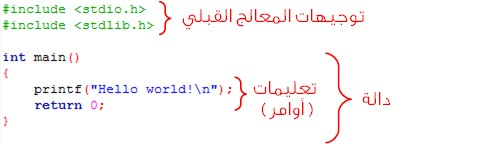
\includegraphics[width=0.8\textwidth]{Chapter_I-3_HelloWorld}
\end{figure}

\subsection{لنجرّب برنامجنا}

كلّ ما سنقوم به الآن هو ترجمة المشروع ثمّ تشغيله (اضغط على
\InlineCode{Build \& Run}
 إذا كنت على
\textenglish{Code::Blocks}).
سيطلب منك حفظ مشروعك إذا لم تقم بذلك من قبل.

\begin{critical}
  إن لم تنجح الترجمة و ظهر لك خطأ مثل :\\
\InlineCode{"My-program - Release" uses an invalid compiler. Skipping...}\\\InlineCode{Nothing to be done...}
فهذا يعني أنّك نزلت نسخة
\textenglish{Code::Blocks}
 دون
\InlineCode{mingw}
 (المترجم)، عد و نزّل النسخة التي تحتوي على
\InlineCode{mingw}.
\end{critical}

بعد بُرهة، يظهر برنامجك كما في الصورة :

\begin{figure}[H]
	\centering
	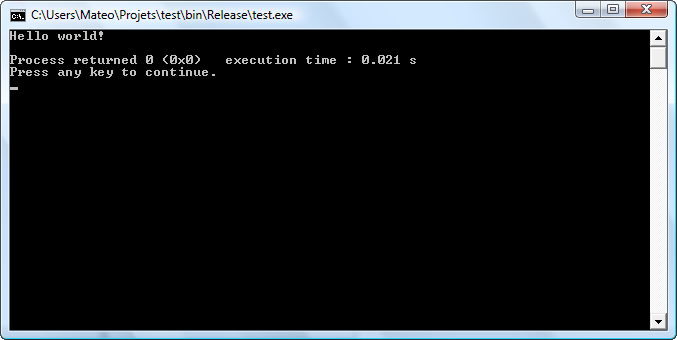
\includegraphics[width=0.8\textwidth]{Chapter_I-3_HelloWorld-run}
\end{figure}

البرنامج يُظهر
"\textenglish{Hello world!}"
 (في السطر الأوّل).\\
الأسطر الّتي أسفله تمّ توليدها من طرف
\textenglish{Code::Blocks}
 وتدلّ على أنّ البرنامج قد تمّ تشغيله بنجاح كما أنها تعطي الوقت الذي استغرقه البرنامج في التشغيل.

 سيطلب منك الضغط على إحدى المفاتيح لإغلاق النافذة. أعلم أن الأمر لم يكن ممتعا جدّا. لكنه برنامجك الأوّل، وهذه لحظة ستتذكرها طيلة حياتك ! ألا تعتقد ذلك ؟

\section{كتابة رسالة على الشاشة}

من الآن سنقوم بإدخال التعديلات على الشفرة المصدرية السابقة. مهمّتك، إن قبلتها : عرض رسالة
"\textenglish{Bonjour}"
 على الشاشة.

\begin{question}
  كيف يمكنني اختيار النص الّذي سيظهر على الشاشة ؟
\end{question}

الأمر بسيط جدا، إذا بدأت من الشفرة التي رأيناها سابقاً، فسيكون عليك استبدال
"\textenglish{Hello world!}"
 بـ"\textenglish{Bonjour}"
 في السطر الذي يستدعي
\InlineCode{printf}.

كما قلت من قبل،
\InlineCode{printf}
 هي
\textbf{تعليمة}
 وهي تعطي أمراً للحاسوب : "قم بعرض هذه الرسالة على الشاشة".\\
يجب أن تعرف أيضا أن
\InlineCode{printf}
 هي دالّة كُتِبَت من قبل من طرف مبرمجين قبلك.

\begin{question}
   أين توجد هذه الدالّة ؟ أنا لا أرى سوى الدالّة \InlineCode{main} !
\end{question}

هل تذكر هذين السطرين ؟

\begin{Csource}
#include <stdio.h>
#include <stdlib.h>
\end{Csource}

قلت لك من قبل أنهما يمكنان البرنامج من إضافة مكتبات. المكتبات في الحقيقة هي ملفّات تحوي أطنانا من الدوال جاهزة للإستخدام. هذه الملفات
(\InlineCode{stdio.h} و \InlineCode{stdlib.h})
 تحوي أغلب الدوال الأساسية التي قد نحتاجها في برنامج ما.
\InlineCode{stdio.h}
 بحد ذاته يحوي دوال تمكّن من عرض أشياء على الشاشة (مثل
 \InlineCode{printf})
 و أيضا الطلب من المستخدم إدخال شيء ما (هذه دوال سنتعرّف عليها لاحقا).

\subsection{لنقل مرحبا للسيّد}

في دالّتنا
\InlineCode{main}
نستدعي الدالّة
 \InlineCode{printf}.
 أي أن لدينا دالّة تستدعي أخرى (هنا
\InlineCode{main}
تستدعي
\InlineCode{printf}).
سترى أن هذا ما يحدث دائما في لغة
\textenglish{C}
: دالّة تحتوي تعليمات تستدعي دوال أخرى، وهكذا.

إذن، لاستدعاء دالّة يكفي كتابة اسمها متبوعا بقوسين، ثم فاصلة منقوطة.

\begin{Csource}
printf();
\end{Csource}

هذا جيد، لكنه غير كاف. يجب أن نُعلم البرنامج بما يجب أن يكتبه في الشاشة. لفعل هذا يجب أن نعطي
\InlineCode{printf}
النص المطلوب عرضه. لفعل هذا نقوم بوضع النص داخل علامات الإقتباس المزدوجة بين القوسين.\\
في حالتنا هذه سنكتب تماما :

\begin{Csource}
printf("Bonjour");
\end{Csource}

آمل ألا تكون قد نسيت رمز الفاصلة المنقوطة في النهاية، وأذكّرك أنّها مهمّة جدا لأنّها تدلّ على نهاية التعليمة.\\
هذه هي الشفرة المصدرية التي يجب أن تحصل عليها :

\begin{Csource}
#include <stdio.h>
#include <stdlib.h>

int main()
{
    printf("Bonjour");
    return 0;
}
\end{Csource}

لدينا إذن تعليمتان تطلبان من الحاسوب القيام بهذين الأمرين بهذا الترتيب :
\begin{enumerate}
  \item عرض
"\textenglish{Bonjour}"
على الشاشة.
  \item نهاية الدالّة
\InlineCode{main}
، إعادة 0. البرنامج يتوقّف.
\end{enumerate}

هذا ما يظهر على شاشتك :

\begin{figure}[H]
	\centering
	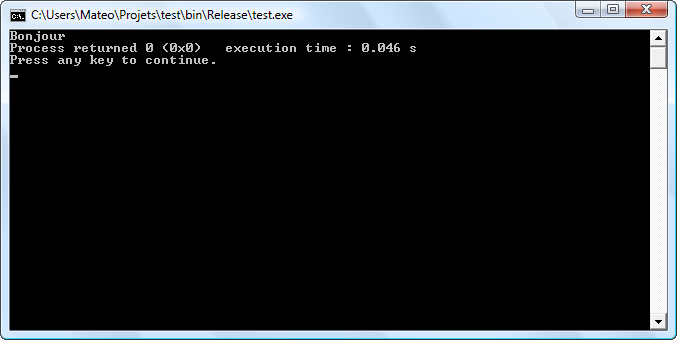
\includegraphics[width=0.8\textwidth]{Chapter_I-3_Good-Morning}
\end{figure}

كما ترى، السطر الذي يحتوي الرسالة يكون ملتصقاً قليلا بباقي النص، على خلاف ما رأيناه سابقا.\\
أحد الحلول الممكنة هو إضافة رمز للعودة إلى السطر بعد
 "\textenglish{Bonjour}"
 (كما لو أنّنا ضغطنا على المفتاح
\InlineCode{Enter}).

ولكن ضغط المفتاح
\InlineCode{Enter}
 في الشفرة المصدرية لن يعمل كما تتوقع، لهذا يجب استخدام المحارف الخاصّة
(\textenglish{Special characters}).

\subsection{المحارف الخاصّة}

المحارف أو الرموز الخاصّة هي محارف تمكّن من تعريف عودة إلى السطر، جدولة، إلخ.\\
من السهل التعرّف عليها، فهي مكوّنة من محرفين. الأوّل هو الشَرْطَةُ المائلة الخلفية 
(\textbackslash) (\textenglish{Backslash})
والثاني يكون رقما أو حرفا. إليك محرفين خاصّين قد تحتاجهما كثيرا :

\begin{itemize}
  \item \InlineCode{\textbackslash n} :
 العودة إلى السطر.
 \item \InlineCode{\textbackslash t} :
 الجدولة (فراغ كبير في نفس السطر).
\end{itemize}

في حالتنا هذه، يكفي أن نكتب
\InlineCode{\textbackslash n}
 لإنشاء العودة إلى السطر. إذن، إذا أردنا أن نضع عودة إلى السطر بعد
\textenglish{Bonjour}
، فيكفي أن نكتب :

\begin{Csource}
printf("Bonjour\n");
\end{Csource}

وسيفهم حاسوبك أنّ عليه كتابة
"\textenglish{Bonjour}"
 ويعود إلى السطر.

\begin{figure}[H]
	\centering
	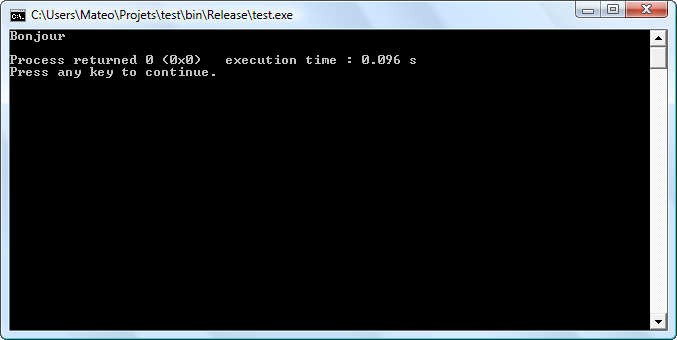
\includegraphics[width=0.8\textwidth]{Chapter_I-3_Good-Morning-backslash-n}
\end{figure}

\begin{information}
  يمكنك الكتابة بعد
\InlineCode{\textbackslash n}
بدون أيّة مشكلة. كلّ ما تكتبه بعد
\InlineCode{\textbackslash n}
 سيوضع في السطر الجديد. يمكنك إذن التدرّب على كتابة :
\InlineCode{printf("Good morning\textbackslash nGood bye\textbackslash n");}\\
و سيتمّ عرض
"\textenglish{Good morning}"
على السطر الأوّل و
"\textenglish{Good bye}"
على السطر الثاني.
\end{information}

\subsection{متلازمة \textenglish{Gérard}}

\begin{question}
  مرحبا، اسمي
\textenglish{Gérard}
و قد حاولت تعديل برنامجك ليقول
"\textenglish{Bonjour Gérard}"،
و لكنّي ألاحظ أنّ حرف
\textenglish{é}
 لا يظهر بشكل جيّد
\dots
 مالّذي عليّ فعله ؟
\end{question}

أوّلا، مرحبا بك
\textenglish{Gérard}
. هذا سؤال جيّد. لكن لديّ خبر سيّء لك. الكونسول الخاصة بـ\textenglish{Windows}
لا تمكّن من عرض الحروف الّتي تحوي علامات النطق الصوتي مثل
\textenglish{é}
، خلافا لكونسول
\textenglish{GNU/Linux}
التي تفعل. لديّ حلّان لهذه المشكلة :

\begin{itemize}
  \item \textbf{استخدم
\textenglish{GNU/Linux}}
. هذا حلّ جذريّ بعض الشيء. أحتاج إلى درس كامل لأعلّمك كيف تعمل على
\textenglish{GNU/Linux}
. إذا لم يكن لديك المستوى، إنس هذا الخيار حاليّا.
  \item \textbf{لا تستخدم الحروف الّتي تحوي علامات النطق الصوتي}.
للأسف إنّه الحل الّذي قد يكون عليك اختياره. الكونسول الخاصة بـ\textenglish{Windows}
لها عيوبها. يجب عليك التعوّد على عدم كتابة مثل هذه الحروف. لكن مستقبلا قد تنشئ برامج بنوافذ ولن تعاني من هذا المشكل. لذلك أنصحك بالصبر على هذه المشكلة حاليّا، فبرامجك المستقبلية "الاحترافية" لن يكون فيها هذا المشكل.
\end{itemize}

لكيلا تنزعج، يمكنك الكتابة دون استخدام الحروف التي تملك علامات النطق الصوتي :

\begin{Csource}
printf("Bonjour Gerard\n");
\end{Csource}

نشكر صديقنا
\textenglish{Gérard}
لتنبيهنا على هذه المشكلة !

\section{التعليقات، مهمّة جدا !}

قبل ختم هذا الفصل الأوّل "الحقيقي" في البرمجة، يجب أن أعرّفك على
\textbf{التعليقات}
(\textenglish{Comments})
. أيّا كانت لغة البرمجة الّتي تستخدمها، ستكون لديك القدرة على إضافة التعليقات للشفرة المصدرية الخاصة بك.

ولكن ما الذي يعنيه "التعليق"؟\\
هذا يعني إمكانية وضع نصّ في وسط برنامجك لشرح دوره، مثلاً : ما الذي يفعله هذا السطر، إلخ. هذا بالفعل أمر ضروريّ، لأنّه حتّى لو كنت عبقرياً في البرمجة، ستكون بحاجة إلى وضع ملاحظات هنا وهناك. هذا يمكنك من :

\begin{itemize}
  \item العثور على ما تبحث عنه بسهولة في الشفرة المصدرية عندما تعود إليه بعد مدّة. من الطبيعيّ أن ننسى كيف تعمل البرامج الّتي كتبناها بعد مدّة. إن توقّفت عن البرمجة لأيّام ثمّ عدت فستكون بحاجة إلى التعليقات لإيجاد ما تريد في شفرة كبيرة جدّا.
  \item إذا أعطيت مشروعك لأحد غيرك (وهو لا يعرف شيئا عن الشفرة المصدرية الخاصة بك)، فالتعليقات تمكّنه من التآلف مع مشروعك بسرعة.
  \item وأخيرا، ستسمح لي بإضافة شروحات وملاحظات حول الشفرة المصدرية في هذه الدروس. وهذا سيفيدك في فهم ما الذي يعنيه كلّ سطر.
\end{itemize}

توجد طريقتان لإضافة تعليق. وهذا يعتمد على طول التعليق المراد إدراجه :

\begin{itemize}
  \item إذا كان تعليقك
\textbf{قصيرا}
: فيمكن كتابته على سطر واحد، ولا يحتوي سوى كلمات قليلة. في هذه الحالة، عليك كتابة شرطتين مائلتين
(\InlineCode{//})
متبوعين بتعليقك. على سبيل المثال :

\begin{Csource}
// This is a comment.
\end{Csource}

بإمكانك إضافة تعليق وحده على السطر، أو على يمين تعليمة معينة. وهذا أمر مهمّ جدّا، لأنّ بهذه الطريقة يمكننا تحديد ما الذي يعنيه السطر الّذي كُتب بجانبه. مثال :

\begin{Csource}
printf("Bonjour"); // This instruction displays 'Bonjour' on the screen
\end{Csource}

  \item  إذا كان تعليقك
\textbf{طويلا}:
لديك الكثير لتقوله، تريد كتابة الكثير من الجمل على كثير من الأسطر. في هذه الحالة، يجب عليك كتابة شفرة تشير إلى "بداية التعليق" وأخرى تشير إلى "نهاية التعليق":

  \begin{itemize}
    \item لبدء التعليق : أكتب شرطة مائلة متبوعة بنجمة 
    (\InlineCode{/*}).
    \item لإنهاء التعليق : أكتب نجمة متبوعة بشرطة مائلة 
    (\InlineCode{*/}).
  \end{itemize}

  يمكنك كتابة هذا على سبيل المثال :
  
  \begin{Csource}
/* This is
a comment
written on several lines */
  \end{Csource}
\end{itemize}
فلنعد إلى الشفرة المصدرية التي تُظهر
"\textenglish{Bonjour}"
على الشاشة ونضيف إليها بعض التعليقات للتدرّب :

\begin{Csource}
/*
Below, the directives of preprocessor.
These lines allow you to add files to your program,
files that we call libraries. Thanks to these libraries, we are ready to use functions for display.
for example, a message on screen.
*/

#include <stdio.h>
#include <stdlib.h>

/*
Following, you have the principal function of the program, called main.
All programs start with this function.
Here, all what does my function is displaying "Bonjour" on the screen.
*/

int main()
{
  printf("Bonjour"); // This instruction displays 'Bonjour' on the screen
  return 0;          // The program returns 0 then it stops.
}
\end{Csource}

هذا هو برنامجنا مع إضافة بعض التعليقات، نعم هو يبدو أكبر نوعا ما، لكنّه في الحقيقة مكافئ للبرنامج السابق. عند الترجمة، كلّ التعليقات يتمّ تجاهلها من طرف المترجم. هذه التعليقات لا تظهر في البرنامج النهائي، فهي تصلح فقط للمبرمجين.

عادة لا نقوم بوضع تعليق لكلّ سطر. لقد قلت وأكرر أنّه من المهم وضع التعليقات في الشفرة المصدرية، لكن يجب عليك معرفة القدر اللازم من التعليقات الواجب وضعه، وضع تعليق في كلّ سطر قد لا يفيد في شيء، بل يضيّع الوقت فقط. مثلا، أنت تعرف أن وظيفة
\InlineCode{printf}
هي عرض نصّ على الشاشة، فلا حاجة لوضع تعليق يشرح ذلك في كلّ مرّة.

من الأحسن التعليق عن عدد من الأسطر دفعة واحدة. هذا يفيد في ذكر وظيفة مجموعة من التعليمات المتتابعة. فيما بعد إن أراد المبرمج إضافة مزيد من التفاصيل في تعليماته، فسيكون بمستوى ذكاء يسمح له بفعل ذلك.

\textbf{تذكر إذن}:
يجب أن تكون التعليقات لإرشاد المبرمج في شفرته المصدرية. حاول التعليق عن مجموعة من الأسطر دفعة واحدة بدل التعليق عن كلّ سطر على حدة.

وإليك هذه المقولة من
\textenglish{IBM} :

\begin{center}
  \itshape\Large
  'إذا قرأت التعليقات الموجودة في برنامج و لم تفهم مبدأ عمله، قم برميه !'
\end{center}

\section*{ملخّص}

\begin{itemize}
  \item البرامج يمكنها التفاعل مع المستخدم عن طريق الكونسول أو عن طريق النافذة.
  \item من السهل على المبرمج في برامجه الأولى استخدام
\textbf{الكونسول}،
رغم أنّ هذه قد تكون غير محبوبة لدى المبتدئ، فهذا لا يمنع من استخدام النوافذ في الجزء الثالث من هذا الكتاب.
  \item البرنامج يتكوّن من
\textbf{تعليمات}
 تنتهي دائما بفاصلة منقوطة.
  \item الدالة
\InlineCode{main}
 (التي تعني الرئيسيّة) هي الدالة الّتي يبدأ بها تنفيذ البرنامج. إنّها الدالة الوحيدة الإجبارية في البرنامج، لا يمكن لأي برنامج أن يُترجم بدونها.
 \item \InlineCode{printf}
 هي دالة تمكننا من عرض رسالة على الشاشة.
 \item \InlineCode{printf}
موجودة في
\textbf{مكتبة}
 تحتوي على كثير من الدوال الأخرى الجاهزة للاستخدام.
\end{itemize}

  \chapter{عالم المتغيّرات}

تعلّمت كيفية إظهار نصّ على الشاشة. جيد، لكنّ هذا ليس شيئا مهماً. هذا لأنك لا تعرف بعد ما يدعى بـ
\underline{المتغيّرات}
(\textenglish{Variables})
في البرمجة.

فائدة هذه المتغيرات هي تمكين الحاسوب من حفظ أعداد في الذاكرة. سنبدأ ببعض الشرح حول ذاكرة الحاسوب وكيفيّة عملها. قد يبدو هذا بسيطا جدّا للبعض، لكنّي أفترض أنّك لا تعرف شيئا عن ذاكرة الحاسوب.

\section{أمر متعلق بالذاكرة}
ما سأعلمك في هذا الدرس هو أمر له علاقة مباشرة بذاكرة حاسوبك.

كل إنسان حيّ له ذاكرة. الأمر عينه بالنسبة للحاسوب، لكن الحاسوب له أنواع عديدة من الذاكرة.

\begin{question}
  لم يملك الحاسوب أنواع عديدة من الذاكرة، واحدة يمكنها أن تكفي، أليس الأمر كذلك؟
\end{question}
كلّا: المشكلة أننا نحتاج ذاكرة سريعة (لاسترجاع المعلومات بسرعة) وفي نفس الوقت كبيرة (لحفظ بيانات كثيرة) قد تضحك إن أخبرتك أننا حتى اليوم لم نتمكن من صنع ذاكرة بهذه المواصفات. أو بالأحرى الذاكرة السريعة باهظة الثمن لذلك لا يتم إنتاج الكثير منها.

لذلك نجد في الحواسيب الحديثة ذاكرة سريعة جدا لكنها ليس ذات سعة كبيرة، وأخرى ذات سعة كبيرة جدّا لكنها غير سريعة.

\subsection{الأنواع المختلفة من الذاكرة}
كي أوضح لك الصورة أكثر، إليك أنواع الذاكرة الموجودة في الحاسوب، من الأسرع إلى الأبطأ:
\begin{enumerate}
  \item السجلات (
\textenglish{Registers}
): ذاكرة سريعة جدّا، موجودة داخل المعالج.
  \item ذاكرة التخبئة (
\textenglish{Cache memory}
): تمثل همزة وصل بين السجلات والذاكرة الحية.
  \item ذاكرة الوصول العشوائي (
\textenglish{Random access memory}
): وهي الذاكرة التي نستخدمها كثيرا، وتدعى اختصارا
\textenglish{RAM}.
  \item القرص الصلب (
\textenglish{Hard disk}
): والذي تعرفه بالطبع، نستعمله لحفظ الملفات.
\end{enumerate}
كما قلت لك، لقد رتبتها من الأسرع (السجلات) إلى الأبطأ (القرص الصلب)، وإن كنت قد تابعت جيدا فقد فهمت أن الذاكرة الأصغر هي الأسرع والأبطأ هي الأكبر.\\
السجلات لا تسع إلا لحمل بضعة أعداد أما القرص الصلب فيمكنه تخزين ملفات ضخمة.

\begin{information}
   عندما أقول ذاكرة بطيئة فهذا بالنسبة لحاسوبك، ففي نظر الحاسوب استغراق 8 ميلي ثانية للوصول إلى القرص الصلب يعتبر زمنا طويلا جدّا!
\end{information}

ما الذي يجب أن أتذكره من كل هذا؟\\
أردت أن أخبرك أننا في الدروس القادمة سوف نستخدم ذاكرة الوصول العشوائي كثيرا. سنتعلم أيضا كيفية القراءة والكتابة في الملفات على القرص الصلب (ليس الآن، لا يزال الوقت مبكّرا على هذا). أمّا بخصوص السجلّات وذاكرة التخبئة فلن نتعامل معهما مطلقا، فالحاسوب هو من سيهتم بأمرهما.

\begin{information}
  في لغات البرمجة منخفضة المستوى، كلغة التجميع (
\textenglish{Assembly language}
) نتعامل مباشرة مع السجلّات، لقد درستها، ويمكنني أن أقول لك أن القيام بعملية ضرب بسيطة يتطلب مجهودا! لحسن الحظ ففي لغة
\textenglish{C}
 (وفي أغلب اللغات الأخرى) الأمر أسهل من ذلك بكثير.
\end{information}

يجب إضافة شيء مهمّ آخر: القرص الصلب هو الوحيد الذي يمكنه حفظ المعلومات بشكل دائم.
\textbf{كل أنواع الذاكرات الأخرى مؤقتة، فبمجرد إطفاء الحاسوب تفقد كل محتواها}!

لحسن الحظ فعند إعادة تشغيل الحاسوب يقوم القرص الصلب بتذكيرها بمحتواها.

\subsection{صورة لذاكرة الوصول العشوائي}
نظرا لأننا سنستعمل ذاكرة الوصول العشوائي خلال لحظات، فمن الأفضل أن أريها لكم (مؤطر بالأحمر):
\Picture{Chapter_I-4_Computer}
لا أطلب منك معرفة كيفية عملها، لكن أردت فقط أن أريك مكانها داخل جهازك. وهذه صورة مقربة لإحدى أشرطتها:
\Picture{Chapter_I-4_RAM}
وهي تدعى اختصارا
\textbf{\textenglish{RAM}}
، لذلك لا تحتر إن سميتها هكذا لاحقا. بالنسبة للذاكرات الأخرى (السجلات والتخبئة) فهي صغيرة لدرجة أنه لا يمكن رؤيتها بالعين المجرّدة.

\subsection{مخطط ذاكرة الوصول العشوائي}
عرض المزيد من الصور لن يفيدك كثيرا، لكن يجب عليك فهم كيف تعمل من الداخل، لذلك سأقدم لك هذا المخطط البسيط الذي يمثل هندسة ذاكرة الوصول العشوائي:
\Picture{Chapter_I-4_RAM-Schema}

كما ترى، يمكننا أن نميز عمودين:
\begin{itemize}
  \item هناك
\textbf{العناوين}
: هي أعداد تسمح للحاسوب بتحديد موضع القيم في الـ
\textenglish{RAM}
. نبدأ بالعنوان 0 وننتهي بالعنوان 3,448,765,900,126 وبعض الأجزاء. لا أعلم بالضبط كم عدد العناوين الموجودة في الـ
\textenglish{RAM}
، لكني أعرف أنها كثيرة جدا. إضافة إلى ذلك، هذا أمر يتعلق بكمية الذاكرة الموجودة في جهازك، فكلما زادت الذاكرة زادت معها العناوين وصار بإمكاننا تخزين معلومات أكثر.
  \item عند كل عنوان يمكننا تخزين
\textbf{قيمة}
(عدد). حاسوبك يقوم بتخزين هذه الأعداد في ذاكرة الوصول العشوائي لكي يتمكن من تذكرها. ولا يمكننا تخزين سوى عدد واحد عند كل عنوان.
\end{itemize}

لا يمكن للذاكرة الحية تخزين شيء سوى الأعداد.

\begin{question}
  لكن كيف يمكننا تخزين الكلمات؟
\end{question}

سؤال جيد. في الواقع حتى الحروف ليست سوى أعداد في نظر الحاسوب! الجملة هي مجرد تتابع لأعداد.\\
يوجد جدول يوافق بين الأعداد والحروف، جدول يقول مثلا بأن العدد 67 يوافق الحرف
\textenglish{Y}
. لن أدخل في التفاصيل أكثر، ستكون لنا فرصة للرجوع إلى هذا لاحقا.

فلنعد إلى مخططنا، الأمور بسيطة جدا: إذا أراد الحاسوب تذكر العدد 5 (الذي قد يمثل عدد الأرواح المتبقية لشخصية في لعبة) فسوف يضعه في مكان ما في الذاكرة أين يتوفر مكان شاغر ويحفظ العنوان الموافق (مثلا 3,062,199,902). لاحقا، عندما يريد معرفة هذا العدد فسيذهب إلى خانة الذاكرة التي تحمل العنوان رقم 3,062,199,902 وسيجد القيمة 5.

هذه آلية عمل الذاكرة بشكل عام. قد يكون الأمر لا زال غامضا في ذهنك حاليا (ما فائدة تخزين عدد إن كان علينا تذكر عنوانه بدلا من ذلك؟) لكن كل شيء سيتضح مع بقية الدروس، أنا أعدك!

\section{التصريح عن متغير}
صدّقني هذه المقدّمة القصيرة عن الذاكرة ستكون مهمّة أكثر مما تعتقد. الآن يمكننا العودة إلى البرمجة.

إذن، ما هو
\underline{المتغير}
(\textenglish{Variable}) ؟\\
إنه معلومة صغيرة نخزنها مؤقتا في الذاكرة الحية. ببساطة يمكننا القول إن المتغير هو قيمة يمكن أن تتغير أثناء اشتغال البرنامج. مثلا عددنا 5 الذي ذكرناه سابقا يمكن أن يتناقص بمرور الزمن. إذا وصل إلى العدد 0 فسنعرف أن اللاعب قد خسر.

في برامجنا سيكون هناك الكثير من المتغيرات. ستراها في كلّ مكان.

في لغة السي، المتغير يتميز بشيئين:
\begin{itemize}
  \item \underline{قيمة}
: هو العدد الذي يحويه، 5 مثلا.
  \item \underline{اسم}
: وهو الذي يمكننا من معرفة المتغيّر. في البرمجة لن يكون علينا تذكّر عناوين الذاكرة. بدلا من ذلك علينا فقط استخدام أسماء المتغيرات. المترجم هو من سيقوم بتحويل الأسماء إلى عناوين.
\end{itemize}

\subsection{إعطاء اسم للمتغير}
في لغة البرمجة
\textenglish{C}
كل متغير يجب أن يملك اسما خاصا به. ومن أجل متغيرنا الذي يحوي عدد الأرواح المتبقية للاعب يمكننا أن نسميه
"\textenglish{Number of lives}"
أو شيء من هذا القبيل.

للأسف توجد بعض الشروط، لا يمكنك تسمية المتغير كيفما شئت:
\begin{itemize}
  \item لا يجب أن يحتوي الاسم سوى على الحروف الصغيرة والكبيرة والأرقام
(\InlineCode{abcABC012}).
  \item يجب أن يبدأ الاسم بحرف.
  \item المسافات ممنوعة. بدلا من ذلك يمكننا استخدام الحرف المعروف باسم
\textenglish{underscore}
 (\InlineCode{\_}).
إنه الحرف الخاص الوحيد غير الحروف والأرقام الذي يمكن استعماله في اسم متغير.
  \item لا يمكنك استخدام حروف غير الحروف الإنجليزية.
\end{itemize}

وأخيرا يجب أن تعرف أن لغة
\textenglish{C}
 تفرّق بين الحروف الصغيرة والكبيرة. ولثقافتك، نقول إن
\textenglish{C}
 حساسة لحالة الأحرف
(\textenglish{Case sensitive}).
كمثال، الأسماء
\InlineCode{width}
 أو
\InlineCode{WIDTH}
 أو
\InlineCode{WiDth}
تعتبر أسماء متغيرات مختلفة، حتى لو كانت تعني لنا الأمر نفسه.

هذه أمثلة عن أسماء متغيرات صالحة:
\InlineCode{numberOfLives}،
\InlineCode{name}،
\InlineCode{surname}،
\InlineCode{phone\_number}،
\InlineCode{phoneNumber}.

لكل مبرمج طريقة خاصة في كتابة أسماء المتغيرات. خلال هذا الدرس سأريك طريقتي:
\begin{itemize}
  \item أبدأ دائما بحرف صغير.
  \item إن كان في الاسم أكثر من كلمة أضع حرف كبيرا في بداية كلّ كلمة.
\end{itemize}

أطلب منك كتابة أسماء متغيراتك بنفس الطريقة التي أتبعها، هذا لكي نكون على تفاهم.

\begin{critical}
  أيّا كان اختيارك، فعليك دائما إعطاء أسماء واضحة لمتغيراتك. كان بإمكاننا اختصار
\InlineCode{numberOfLives}
إلى
\InlineCode{nol}
مثلا. هذا أقصر في الكتابة، لكنه أقل وضوحا عندما تعيد قراءة الشفرة المصدرية. فأنصحك بإعطاء أسماء أطول لمتغيراتك إن كان ذلك يحسّن فهمها.
\end{critical}

\subsection{أنواع المتغيرات}
حاسوبنا كما نعلم ليس سوى آلة كبيرة جدا للحساب. لا يجيد التعامل سوى مع الأعداد. لكن يوجد أنواع كثيرة من الأعداد:
\begin{itemize}
  \item الأعداد الصحيحة الموجبة (الطبيعية) مثل :45، 398، 7650.
  \item الأعداد العشرية، أي التي تحوي فاصلة عشرية: 75.909، 1.7741، 9810.7.
  \item الأعداد الصحيحة السالبة: -87، -916.
  \item الأعداد العشرية السالبة: -76.9، -100.11.
\end{itemize}

حاسوبك المسكين بحاجة للمساعدة! عندما تطلب منه تخزين عدد، يجب أن تذكر له نوعه. هذا ليس لأنّه لا يمكنه التعرف عليه تلقائيّا، ولكن للتنظيم ولعدم أخذ كميات كبيرة من الذاكرة بدون فائدة.

عندما تصرّح عن متغيّر فسيكون عليك تحديد نوعه. إليك أنواع المتغيرات الأساسية في لغة \textenglish{C}:

\begin{Table}{3} % The number of columns is required (here is 3)
  النوع & الحد الأدنى & الحد الأقصى\\
  \LR{\ttfamily signed char} & $-128$ & $127$ \\
  \LR{\ttfamily int} & $-32,768$ & $32,767$ \\
  \LR{\ttfamily long} & $-2147483648$ & $2147483647$ \\
  \LR{\ttfamily float} & $-1 \times 10^{37}$ & $1 \times 10^{37}-1$\\
  \LR{\ttfamily double} & $-1 \times 10^{37}$ & $1 \times 10^{37}-1$\\
\end{Table}

\begin{warning}
  القيم المعروضة هنا تمثل الحد الأدنى المضمون من طرف اللغة. في الحقيقة قد تتمكن من تخزين أعداد أكبر من هذه. في كلّ الأحوال من المستحسن تذكّر هذه القيم عندما تختار نوع متغيراتك.
\end{warning}

\begin{information}
  للعلم أنّي لم أعرض جميع الأنواع هنا، بل الأساسية منها فقط.
\end{information}

الأنواع الثلاثة الأولى
(\InlineCode{char}، \InlineCode{int}، \InlineCode{long})
تسمح يتخزين الأعداد الصحيحة (1،2،3،4،...).\\
النوعان الأخيران
(\InlineCode{float}، \InlineCode{double})
يسمحان بتخزين الأعداد العشرية (13.8, 16.911…).

سترى أنّنا نتعامل من الأعداد الصحيحة معظم الوقت لأنّها سهلة الإستخدام.

\begin{critical}
  احذر في الأعداد العشرية من استخدام الفاصلة، حاسوبك لا يستخدم سوى النقطة. لذلك لا تكتب
$54,9$
 بدل
$54.9$!
\end{critical}

هذا ليس كلّ شيء، توجد أنواع أخرى تعرف بـ
\InlineCode{unsigned}
 (عديمة الإشارة) تصلح لتخزين الأعداد الموجبة فقط. يجب إضافة كلمة
\InlineCode{unsigned}
إلى النوع لاستخدامها.

\begin{Table*}{2}
  \LR{\ttfamily unsigned char} & من
$0$
 إلى
$255$ \\
  \LR{\ttfamily unsigned int} & من
$0$
إلى
$65,535$ \\
  \LR{\ttfamily unsigned int} & من
$0$
إلى
$4,294,967,295$\\
\end{Table*}

كما ترى، مشكلة الأنواع عديمة الإشارة هي عدم القدرة على تخزين الأعداد السالبة، لكن الشيء الإيجابي هي أنّها توفّر لنا ضعف حجم التخزين لكلّ نوع موافق (مثلا
\InlineCode{signed char}
يتوقّف عند 127، بينما
\InlineCode{unsigned char}
يمتد إلى 255.

\begin{information}
  تلاحظون أنّ النوع
\InlineCode{char}
قد تمّ إدراجه إمّا مع الكلمة المفتاحية
\InlineCode{signed}
،أو مع الكلمة المفتاحية
\InlineCode{unsigned}
لكن لا يوضع وحده أبدا. السبب بسيط: هذا النوع يمكن أن يكون بإشارة أو بدون إشارة حسب الحواسيب. لذلك أنصحكم بتحديد أي واحد منهما تريدون حسب نوع القيمة المراد تخزينها.
\end{information}

\begin{question}
  لم توجد ثلاثة أنواع من المتغيرات الصحيحة ؟ ألا يكفي نوع واحد ؟
\end{question}

بلى، و لكن إنشاء أنواع متعدّدة هدفه الاقتصاد من استهلاك الذاكرة. فعندما نطلب من الحاسوب حجز مساحة لمتغيّر من نوع
\InlineCode{char}
فهذا سيكون أقل من المساحة المستهلكة لو إخترنا متغيّرا من نوع
\InlineCode{int}.

كان هذا مهمّا جدّا عندما كانت الحواسيب محدودة الذاكرة. أمّا اليوم فحواسيبنا بها ذاكرات كبيرة جدّا فلم يعد هذا يمثّل مشكلة. إذا احترت أيّ واحد من الأنواع تستخدم، فاختر
\InlineCode{int}
للأعداد الصحيحة (أو
\InlineCode{double}
للعشرية).

باختصار، نقوم بالتفريق خاصّة بين الأعداد الصحيحة و العشريّة
\begin{itemize}
  \item بالنسبة للأعداد الصحيحة، نستعمل عادة
\InlineCode{int}.
  \item بالنسبة للأعداد العشريّة نستعمل عادة
\InlineCode{double}.
\end{itemize}

\subsection{التصريح عن متغيّر}
ها قد بدأنا. الآن سنقوم بإنشاء برنامج كونسول نسميه "\textenglish{variables}".\\
 سنتعلم كيف نصرّح عن متغيّر، أي
 \textbf{الطلب من الحاسوب إذنا باستخدام شيء من ذاكرة الوصول العشوائي}.

 التصريح سيكون سهلا الآن، يجب علينا فقط أن نتّبع الترتيب التالي :
 \begin{enumerate}
   \item نحدّد نوع المتغيّر المراد إنشائه.
   \item نترك فراغا.
   \item نحدد اسم المتغيّر.
   \item و أخيرا، يجب ألاّ ننسى أبدا وضع الفاصلة المنقوطة.
 \end{enumerate}

 مثلا، إذا أردنا إنشاء المتغيّر
\InlineCode{numberOfLives}
 من نوع
\InlineCode{int}
سنكتب السطر التالي :
\begin{Csource}
int numberOfLives;
\end{Csource}

هذا كل ما في الأمر، وإليك بعض الأمثلة الغبيّة لملاحظة الشكل:
\begin{Csource}
int mathMark;
double moneySumReceived;
unsigned int numberOfReadersWhoAreReadingALongVariableName;
\end{Csource}
حسنا، أعتقد أنّك فهمت المبدأ الآن !

ما فعلناه للتو يسمّى
\underline{تصريحا عن متغيّر}
(\textenglish{Declaring a variable})
(هذا مصطلح يجب حفظه). يمكنك وضع التصريحات في بدايات الدوال. و بما أن لدينا دالّة وحيدة فقط
(الدالة
\InlineCode{main})
فسنصرّح المتغيّر هكذا :
\begin{Csource}
#include <stdio.h>
#include <stdlib.h>

int main(int argc, char *argv[]) // Equivalent to int main()
{
  int numberOfLives;

  return 0;
}
\end{Csource}
إن قمتم بتشغيل البرنامج فستلاحظ بدهشة ... أنّه لا يقوم بشيء.

\subsection{بعض التوضيحات}
في الواقع، هناك أشياء تحدث، لكنّك لا تراها. عندما يصل البرنامج إلى سطر التصريح عن المتغيّر فإنّه يطلب من الحاسوب بهدوء أن يعطيه شيئا من ذاكرة الوصول العشوائي.\\
إن تم كلّ شيء على أحسن حال (و هذا ما يقع في غالب الأحيان) فإن الحاسوب يوافق على هذا الطلب.
المشكل الوحيد الذي يمكن أن يقع هو امتلاء الذاكرة، لكنّ هذا أمر نادر الحدوث، من الذي سيملؤ الذاكرة بمتغيرات
\InlineCode{int}
 ؟

لذلك كن متيقناً أنه سوف يتم إنشاء المتغيرات بنجاح.

\begin{information}
  معلومة صغيرة : إن كان لديك عدد من المتغيّرات بنفس النوع تريد التصريح عنها، فمن غير الضروري كتابة سطر لكلّ متغيّر. يكفي فصل أسماء المتغيّرات عن بعضها بفواصل على نفس السطر، مثلا :
\InlineCode{int numberOfLives, level, playerAge;}.
هذا ينشئ ثلاثة متغيّرات أسماؤها على التوالي :
\InlineCode{numberOfLives}، \InlineCode{level}
و
\InlineCode{playerAge}.
\end{information}

و الآن يجب علينا إعطاء قيمة للمتغيّر الذي أنشأناه.

\subsection{إسناد قيمة إلى متغيّر}
هذا أمر سهل للغاية فإن أردنا أن نعطي قيمة لمتغيرنا
\InlineCode{numberOfLives}
فيكمننا ببساطة كتابة هذا
\begin{Csource}
numberOfLives = 5;
\end{Csource}
لن نفعل شيئا بعد هذا. ستضع إسم المتغير، إشارة تساوي ، بعدها القيمة التي تريد أن تضعها بالداخل، في هذه الحالة سنعطي القيمة 5 للمتغير
\InlineCode{numberOfLives}
. برنامجنا الكامل سيكون هكذا :
\begin{Csource}
#include <stdio.h>
#include <stdlib.h>

int main(int argc, char *argv[]) // Equivalent to int main()
{
  int numberOfLives;
  numberOfLives = 5;

  return 0;
}
\end{Csource}
هنا أيضا لا شيء يُعرض على الشاشة، كلّ شيء يحدث في الذاكرة.\\
في أعماق الحاسوب هناك خانة ذاكرة تأخذ القيمة 5. أليس شيئا رائعا ؟

يمكننا أن نستمتع بتغيير القيمة :
\begin{Csource}
int numberOfLives;
numberOfLives = 5;
numberOfLives = 4;
numberOfLives = 3;
\end{Csource}
في هذا المثال، المتغير سيأخذ القيمة 5 ثم 4 ثم 3. و بما أنّ الحاسوب سريع جدّا ففي أقلّ من رمشة عين يأخذ المتغيّر القيم 5 ثمّ 4 ثمّ 3 ثمّ ينتهي البرنامج.

\subsection{قيمة متغيّر جديد}
هناك سؤال مهمّ يجب أن أطرحه عليك :
\begin{question}
  عند التصريح عن متغيّر، أيّ قيمة تكون فيه ؟
\end{question}
عندما يقرأ الحاسوب هذا السطر
\begin{Csource}
int numberOfLives;
\end{Csource}
فسيحجز مكانا في الذاكرة لهذا المتغيّر، لكن ما هي قيمته في هذه اللحظة ؟\\
هل يملك قيمة افتراضيّة ؟ (0 مثلا).

الجواب هو لا، لا و لا ثمّ لا ! لا توجد قيمة افتراضيّة. المكان محجوز لكنّ القيمة لا تتغيّر. لا يتمّ حذف ما يوجد في خانة الذاكرة. ستكون قيمة متغيّرك هي نفس القيمة التي كانت موجودة من قبل في تلك الخانة، و
\textbf{يمكن أن تكون أيّ شيء} !

إن لم يتم تغيير هذا المكان من الذاكرة من قبل، فقد تكون قيمته 0، لكنّ هذا ليس مؤكّدا، قد يأخد متغيّرك القيمة 363 أو 18، و هذا يدلّ على بقايا برنامج قد استخدم هذه الخانة من قبل.\\
و لهذا كي لا تعترضنا المشاكل لاحقا يجب تهيئة المتغير عند التصريح عنه، في لغة
\textenglish{C}
هذا أمر ممكن حيث أنّ كل ما يجب القيام به هو الدمج بين التصريح و تعيين قيمة المتغير في نفس التعليمة كالتالي :
\begin{Csource}
int numberOfLives = 5;
\end{Csource}
هنا يتمّ  التصريح عن المتغيّر ثمّ إسناد قيمة 5 له بطريقة مباشرة.\\
الشيء الإيجابي هنا أننا متأكدون من أنّ المتغيّر يحمل القيمة 5 مبدئيّا.

\subsection{الثوابت}
قد نريد أحيانا إنشاء متغيّر يحمل قيمة ثابتة طوال وقت تشغيل البرنامج. هذا يعني أنّه بمجرّد التصريح عنه، فإنّه يحافظ على قيمته و لا يمكن لأحد تغيير قيمته التي يحويها.

هذا النوع الخاص من المتغيّرات يسمى الثوابت (\textenglish{Constants})، طبعا هذا لأنّ قيمتها تبقى ثابتة.

للتصريح عن ثابت، تكفي إضافة كلمة
\InlineCode{const}
قبل نوع المتغيّر. و لكن يجب إعطاء الثابت قيمة بمجرّد التصريح عنه، لأنّه لاحقا سيكون الوقت متأخّرا و لن نتمكّن من تغيير قيمته.

مثال على التصريح بثابت :
\begin{Csource}
const int INITIAL_NUMBER_OF_LIVES = 5;
\end{Csource}
\begin{information}
  ليس من الضروري أن يكون اسم الثابت مكوّنا من أحرف كبيرة فقط، لكنّ هذا يساعدنا على التفريق بينها و بين المتغيّرات. لاحظ أيضا أننا نستخدم الرمز
\_
 بدلا من الفراغ.
\end{information}
بغضّ النظر عن هذا، الثابت يستعمل بشكل عادي كالمتغير ، يمكنك عرض قيمته إن أردت. الفرق الوحيد هو أنّه إذا حاولت تغيير قيمة الثابت في برنامجك فسينبّهك المترجم إلى وجود خطأ.

أخطاء الترجمة تعرض أسفل الشاشة (في المكان الذي أسميه "منطقة الموت" هل تتذكر ؟)، في هذه الحالة سيقوم المترجم بعرض رسالة تشبه التالي :\\
\InlineCode{[Warning] assignment of read-only variable 'INITIAL\_NUMBER\_OF\_LIVES'}

\section{عرض محتوى متغير}
نحن نعرف كيف نعرض نصّا على الشاشة باستخدام الدالة
\InlineCode{printf}.\\
الآن سنتعلم كيف نعرض القيمة الخاصة بالمتغير باسخدام نفس الدالة.

سنستخدم الدالة
\InlineCode{printf}
بنفس الطريقة، باستثناء أننا سنقوم بإضافة رمز خاص في المكان الّذي نريد عرض قيمة المتغيّر فيه. مثلا :
\begin{Csource}
printf("You have %d lives left");
\end{Csource}
هذا الرمز الخاص ما هو إلّا
\InlineCode{\%}
 متبوعا بحرف (
\InlineCode{'d'}
في هذا المثال). هذا الحرف يبيّن ما الذي سنقوم بعرضه.
\InlineCode{'d'}
تعني أننا سنعرض قيمة متغيّر من نوع
\InlineCode{int}.\\
توجد حروف أخرى عديدة، لكن من أجل التبسيط فسنكتفي بهذه :
\begin{Table}{2}
الشكل & النوع المنتظر\\
\LR{\ttfamily \%d} & \LR{\ttfamily int}\\
\LR{\ttfamily \%ld} & \LR{\ttfamily long}\\
\LR{\ttfamily \%f} & \LR{\ttfamily float}\\
\LR{\ttfamily \%f} & \LR{\ttfamily double}\\
\end{Table}
\begin{information}
  لاحظوا أنّ الشكل المستخدم لعرض
\InlineCode{float}
و
\InlineCode{double}
هو نفسه.
\end{information}
سأعلّمك رموزا أخرى في الوقت المناسب، حاليّا تذكّر هذه فقط.

شارفنا على الإنتهاء. حددنا موضع كتابة عدد صحيح، لكننا لم نذكر ما هو ! يجب علينا أن نحدد للدالة
\InlineCode{printf}
المتغيّر الذي نريد عرض قيمته.\\
لفعل ذلك، أكتب اسم المتغيّر بعد علامات الاقتباس بعد وضع فاصلة :
\begin{Csource}
printf("You have %d lives left", numberOfLives);
\end{Csource}
\InlineCode{\%d}
 سيتمّ استبداله بقيمة المتغيّر المكتوب بعد الفاصلة، أي
\InlineCode{numberOfLives}.\\
فلنجرّب هذا في برنامج :
\begin{Csource}
#include <stdio.h>
#include <stdlib.h>

int main(int argc, char *argv[])
{
  int numberOfLives = 5; // The player has 5 lives in the beginning.

  printf("You have %d lives left\n", numberOfLives);
  printf("**** B A M ****\n"); // A big blow on his head.
  numberOfLives = 4; // Life lost
  printf("Sorry, only %d lives are remaining now !\n\n", numberOfLives);

  return 0;
}
\end{Csource}
يمكن أن يكون البرنامج قاعدة للعبة فيديو (ينقصه الخيال فقط).\\
هذا البرنامج يعرض على الشاشة :
\begin{Console}
You have 5 lives left
**** B A M ****
Sorry, only 4 lives are remaining now !

\end{Console}
يجب أن تفهم ما الذي يحدث في البرنامج :
\begin{enumerate}
  \item في البداية يملك اللاعب 5 أرواح، نعرض هذا في
\InlineCode{printf}.
  \item  بعدها يتلقى اللاعب ضربة على رأسه (في مكان
\textenglish{BAM}).
  \item بعدها لا يبقى له سوى 4 أرواح، نعرض هذا أيضا باستخدام
\InlineCode{printf}.
\end{enumerate}
كان ذلك سهلا !

\subsection{عرض عدّة متغيّرات باستخدام
\texttt{printf}
واحدة
}
يمكن عرض قيم متغيرات عديدة بنفس الدالة
\InlineCode{printf}.
يكفي فقط أن تضع
\InlineCode{\%d}
أو
\InlineCode{\%f}
 في الأمكنة المناسبة، ثم تحديد المتغيّرات الموافقة بنفس الترتيب، مفصولة عن بعضها البعض بفواصل.

مثال :
\begin{Csource}
printf("You have %d lives and you are in the level n° %d", numberOfLives, level);
\end{Csource}
\begin{warning}
  يجب عليك تحديد المتغيّرات بالترتيب الصحيح،
\InlineCode{\%d}
الأولى توافق المتغيّر الأوّل
(\InlineCode{numberOfLives})
و
\InlineCode{\%d}
الثانية توافق المتغيّر الثاني
(\InlineCode{level}).
إذا أخطأت في الترتيب، فلن يكون للجملة أيّ معنى.
\end{warning}
حسنا، فلنقم بتجربة صغيرة الآن. لاحظ أنني قد حذفت توجيهات المعالج القبلي (أعني تلك السطور التي تبدأ برمز
\InlineCode{\#}
)، أنا أفترض أنك تضعها في كلّ مرّة الآن :
\begin{Csource}
int main(int argc, char *argv[])
{
  int numberOfLives = 5, level = 1;

  printf("You have %d lives and you are in the level n° %d", numberOfLives, level);

  return 0;
}
\end{Csource}
و هذا يعرض لكم :
\begin{Console}
You have 5 lives and you are in the level n° 1
\end{Console}

\end{document}
